\section{Ejercicio 2: Guardando Datos} 

\textbf{}\\
\textbf{}\\
Paso 1. Agregar al proyecto de pruebas una clase de pruebas TestUnit02

\begin{center}
	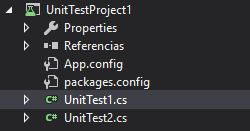
\includegraphics[width=10cm]{./Imagenes/Captura8} 
	\end{center}
\textbf{}\\

Paso 2. Agregar el método InsertarEstudianteSatisfactoriamente, tomar como referencia el siguiente código
\begin{center}
	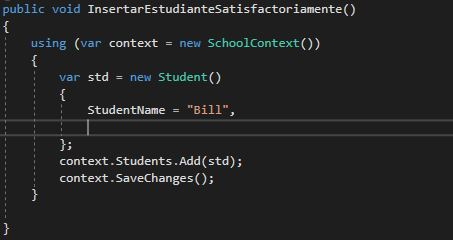
\includegraphics[width=10cm]{./Imagenes/Captura9} 
	\end{center}

\textbf{}\\
La sentencia SQL generada del lado del gestor de base de datos es:
\begin{center}
	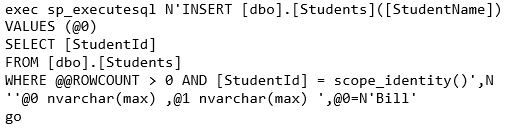
\includegraphics[width=10cm]{./Imagenes/U1-7} 
	\end{center}

\textbf{}\\
Paso 3. Agregar el método ActualizarAlPrimerEstudianteSatisfactoriamente, tomar como referencia el siguiente código
\begin{center}
	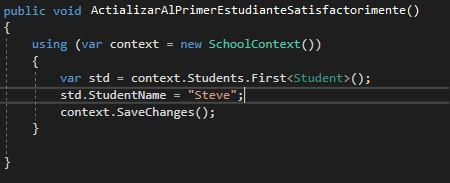
\includegraphics[width=10cm]{./Imagenes/Captura13} 
	\end{center}
\textbf{}\\
La sentencia SQL generada del lado del gestor de base de datos es:

\begin{center}
	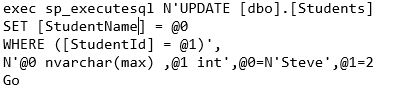
\includegraphics[width=10cm]{./Imagenes/U1-6} 
	\end{center}
\textbf{}\\
Paso 4. Agregar el método EliminarElPrimerEstudianteSatisfactoriamente, tomar como referencia el siguiente
código

\begin{center}
	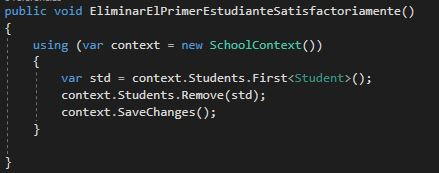
\includegraphics[width=10cm]{./Imagenes/Captura10} 
	\end{center}

\textbf{}\\
La sentencia SQL generada del lado del gestor de base de datos es:
\begin{center}
	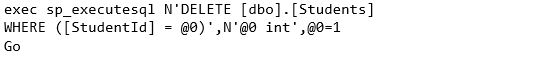
\includegraphics[width=10cm]{./Imagenes/U2-2} 
	\end{center}
\textbf{}\\
Paso 5. Agregar el método: AgregarTresEstudiantesSatisfactoriamente, tomar como referencia el siguiente código:

\begin{center}
	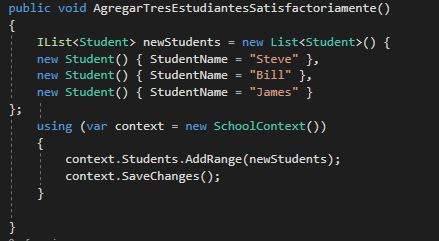
\includegraphics[width=10cm]{./Imagenes/Captura11} 
	\end{center}

\textbf{}\\
Paso 5. Finalmente agregar el método de pruebas: EliminarTresEstudiantesSatisfactoriamente, tomar como
referencia el siguiente código:

\begin{center}
	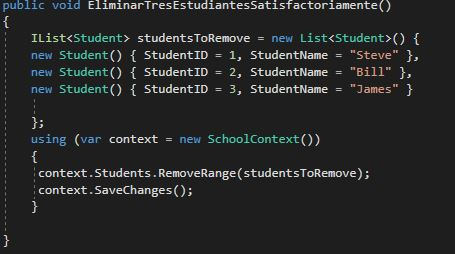
\includegraphics[width=10cm]{./Imagenes/Captura12} 
	\end{center}
\textbf{}\\



